\chapter*{Resultados}
\section*{Resumen}
En este apartado se presentan los resultados obtenidos de la caracterización de cada bloque funcional desarrollado en el marco del proyecto, así como del sistema completo integrado. Se contrasta el desempeño de los prototipos con los valores teóricos calculados y las simulaciones, analizando las diferencias y evaluando el cumplimiento global de las especificaciones técnicas iniciales.

\section*{Sistema de alimentación}

La etapa de alimentación del sistema está basada en el regulador de tensión lineal LM7805, encargado de suministrar una tensión continua regulada y estable de $5~\mathrm{V}$ a los distintos subsistemas de control y procesamiento digital.


\begin{table}[H]
\centering
\begin{tabular}{lcc}
\hline
\textbf{Parámetro} & \textbf{Diseño / Teórico} & \textbf{Valor Medido} \\
\hline
Tensión de entrada ($V_{\text{in}}$) & $8{,}0\text{ a }12{,}0~\mathrm{V}$ & $9{,}0~\mathrm{V}$ \\
Tensión de salida ($V_{\text{out}}$) & $5{,}0~\mathrm{V}$ & $5{,}02~\mathrm{V}$ \\

Riple de salida ($V_{\text{pp}}$) & $< 10~\mathrm{mV}$ & $\approx 6~\mathrm{mV}$ \\
Corriente máxima de salida & $1{,}0~\mathrm{A}$ & $80~\mathrm{mA}$ \\
\hline
\end{tabular}
\caption{Comparación entre los valores de diseño y medidos de la etapa de alimentación.}
\label{tab:resultados_alimentacion}
\end{table}

La etapa de alimentación cumple satisfactoriamente con los requerimientos de estabilidad y bajo nivel de ruido, garantizando una tensión de polarización constante que evita la propagación de fluctuaciones hacia los osciladores y circuitos sensibles de radiofrecuencia.

\section*{Filtro Hairpin}

Las mediciones se enfocaron en la obtención de los parámetros de dispersión $S_{11}$ y $S_{21}$ dentro de la banda de interés.

En la Figura~\ref{fig:hairpin_medicion} se presentan los resultados obtenidos experimentalmente.

\begin{figure}[H]
    \centering
    \begin{subfigure}[b]{0.48\linewidth}
        \centering
        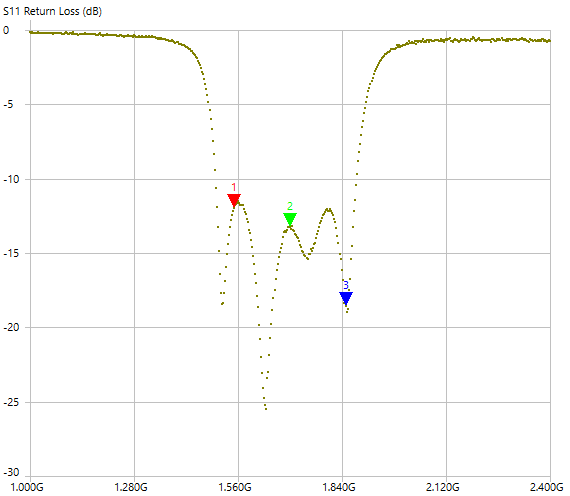
\includegraphics[width=\linewidth]{imagenes/s11.png}
        \caption{$S_{11}$ medido.}
        \label{fig:hairpin_s11}
    \end{subfigure}
    \hfill
    \begin{subfigure}[b]{0.48\linewidth}
        \centering
        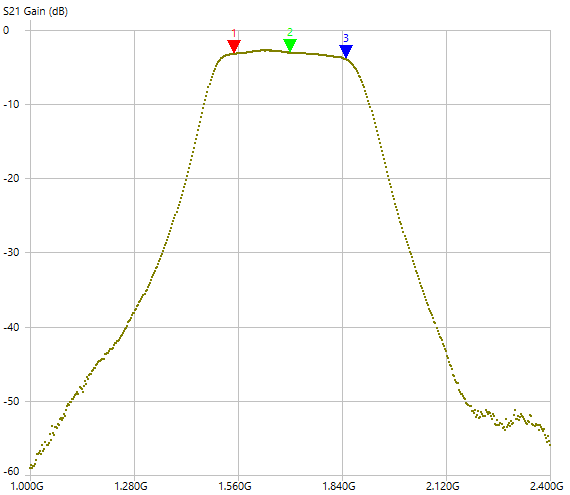
\includegraphics[width=\linewidth]{imagenes/s21.png}
        \caption{$S_{21}$ medido.}
        \label{fig:hairpin_s21}
    \end{subfigure}
    \caption{Parámetros de dispersión medidos para el filtro Hairpin. (Fuente: Propia).}
    \label{fig:hairpin_medicion}
\end{figure}

\begin{table}[H]
\centering
\begin{tabular}{lcc}
\hline
\textbf{Parámetro} & \textbf{Especificación / Diseño} & \textbf{Valor Medido} \\
\hline
Frecuencia central ($f_0$) & $1{,}7~\mathrm{GHz}$ & $1{,}689~\mathrm{GHz}$ \\
Ancho de banda ($BW$) & $390~\mathrm{MHz}$ & $394~\mathrm{MHz}$ \\
Ancho de banda fraccional ($\mathrm{FBW}$) & $0{,}2294$ & $0{,}233$ \\
Frecuencia inferior ($f_1$) & $1{,}505~\mathrm{GHz}$ & $1{,}49~\mathrm{GHz}$ \\
Frecuencia superior ($f_2$) & $1{,}895~\mathrm{GHz}$ & $1{,}886~\mathrm{GHz}$ \\
Rizado de la banda de paso & $0{,}5~\mathrm{dB}$ & $0{,}8~\mathrm{dB}$ \\
Pérdidas de inserción & $< -2~\mathrm{dB}$ & $-4~\mathrm{dB}$ \\
Atenuación a $1{,}35~\mathrm{GHz}$ & $-30~\mathrm{dB}$ & $-30{,}92~\mathrm{dB}$ \\
\hline
\end{tabular}
\caption{Comparación entre las especificaciones de diseño y los valores medidos del filtro Hairpin.}
\label{tab:comparacion_hairpin}
\end{table}

El bloque cumple con su objetivo principal de suprimir las frecuencias indeseadas de arranque y atenuar las componentes fuera de banda. A pesar de un leve desplazamiento en frecuencia y de pérdidas de inserción de $-4~\mathrm{dB}$, el comportamiento obtenido se considera aceptable al mantenerse un bajo rizado ($0{,}8~\mathrm{dB}$) sin afectar la transmisión del \textit{chirp}.

\section*{Divisor de potencia Wilkinson}

La caracterización experimental del divisor de potencia Wilkinson se llevó a cabo mediante un analizador de redes vectorial, obteniéndose los parámetros de dispersión en el intervalo de frecuencias de interés.

En la Figura~\ref{fig:wilkinson_mediciones} se presentan los resultados obtenidos experimentalmente.

\begin{figure}[H]
    \centering
    \begin{subfigure}[b]{0.48\linewidth}
        \centering
        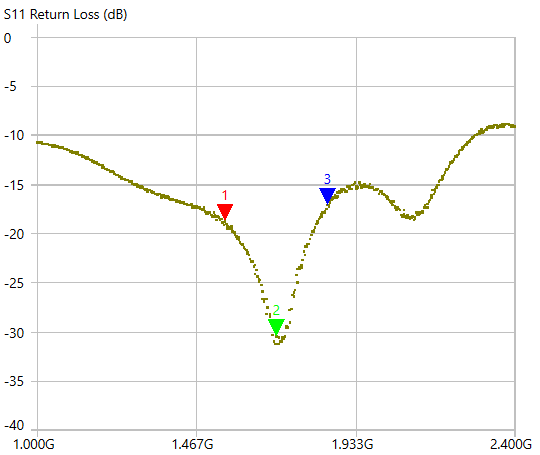
\includegraphics[width=\linewidth]{imagenes/s11_medido.png}
        \caption{$S_{11}$ medido.}
        \label{fig:s11_medido}
    \end{subfigure}
    \hfill
    \begin{subfigure}[b]{0.48\linewidth}
        \centering
        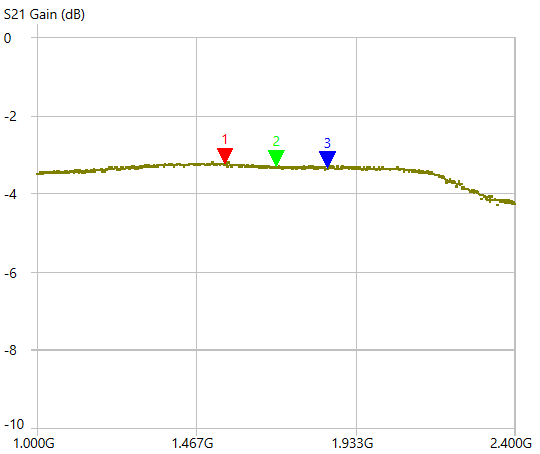
\includegraphics[width=\linewidth]{imagenes/s21_medido.png}
        \caption{$S_{21}$ medido.}
        \label{fig:s21_medido}
    \end{subfigure}

    \vspace{0.5cm}

    \begin{subfigure}[b]{0.48\linewidth}
        \centering
        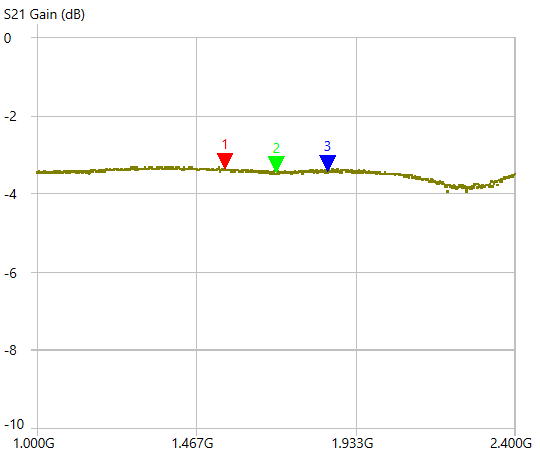
\includegraphics[width=\linewidth]{imagenes/s31_medido.png}
        \caption{$S_{31}$ medido.}
        \label{fig:s31_medido}
    \end{subfigure}
    \hfill
    \begin{subfigure}[b]{0.48\linewidth}
        \centering
        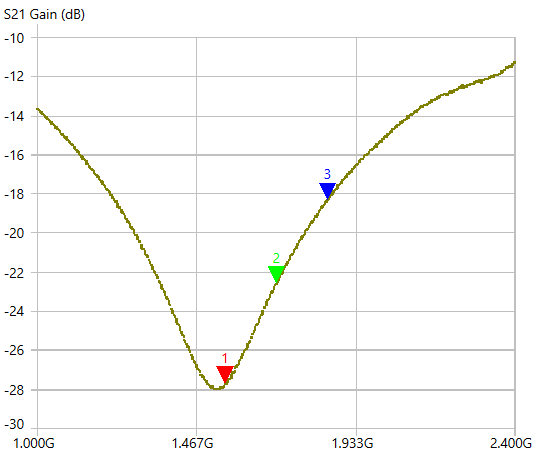
\includegraphics[width=\linewidth]{imagenes/s23_medido.png}
        \caption{$S_{23}$ medido.}
        \label{fig:s23_medido}
    \end{subfigure}

    \caption{Parámetros de dispersión medidos experimentalmente para el divisor de potencia Wilkinson. (Fuente: Propia).}
    \label{fig:wilkinson_mediciones}
\end{figure}

\begin{table}[H]
\centering
\begin{tabular}{lcc}
\hline
\textbf{Parámetro} & \textbf{Simulado} & \textbf{Medido} \\
\hline
$S_{11}$ & $-40~\mathrm{dB}$ & $-30~\mathrm{dB}$ \\
$S_{21}$ & $-3{,}19~\mathrm{dB}$ & $-3{,}33~\mathrm{dB}$ \\
$S_{31}$ & $-3{,}22~\mathrm{dB}$ & $-3{,}48~\mathrm{dB}$ \\
$S_{23}$ & $-37~\mathrm{dB}$ & $-22{,}6~\mathrm{dB}$ \\
Impedancia puerto 2 ($Z_2$) & $50~\Omega$ & $49{,}2 + j7{,}6~\Omega$ \\
Impedancia puerto 3 ($Z_3$) & $50~\Omega$ & $53{,}0 + j0{,}6~\Omega$ \\
\hline
\end{tabular}
\caption{Comparación entre los resultados simulados y medidos del divisor Wilkinson.}
\label{tab:resultados_wilkinson}
\end{table}

El divisor de potencia cumple adecuadamente con la división equitativa de la señal, presentando pérdidas de inserción muy próximas al límite teórico y un buen nivel de adaptación de entrada y aislamiento entre salidas, lo que valida su desempeño en la arquitectura de radiofrecuencia.

\section*{VCO}

La caracterización experimental del módulo VCO a lazo abierto permitió evaluar la sensibilidad de sintonía real ($K_V$), el nivel de espurios, el espectro de la señal y el ruido de fase.

En la Figura~\ref{fig:vcolazoabi} se muestra la medición del VCO a lazo abierto y en la Figura~\ref{fig:medicionrampa} se presenta la rampa de frecuencia obtenida frente al comportamiento ideal.

\begin{figure}[H]
    \centering
    \begin{subfigure}[b]{0.48\linewidth}
        \centering
        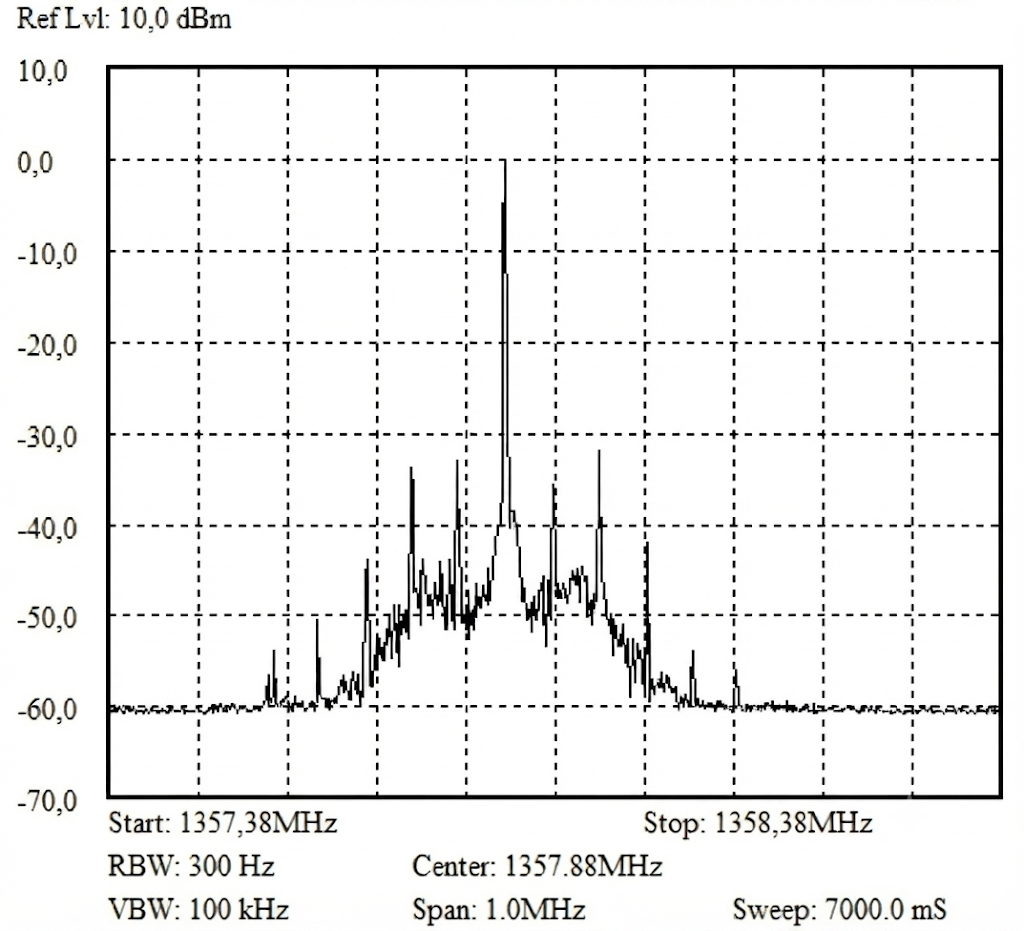
\includegraphics[width=\linewidth]{imagenes/vcomedicionanalizador.png}
        \caption{Medición del VCO a lazo abierto.}
        \label{fig:vcolazoabi}
    \end{subfigure}
    \hfill
    \begin{subfigure}[b]{0.48\linewidth}
        \centering
        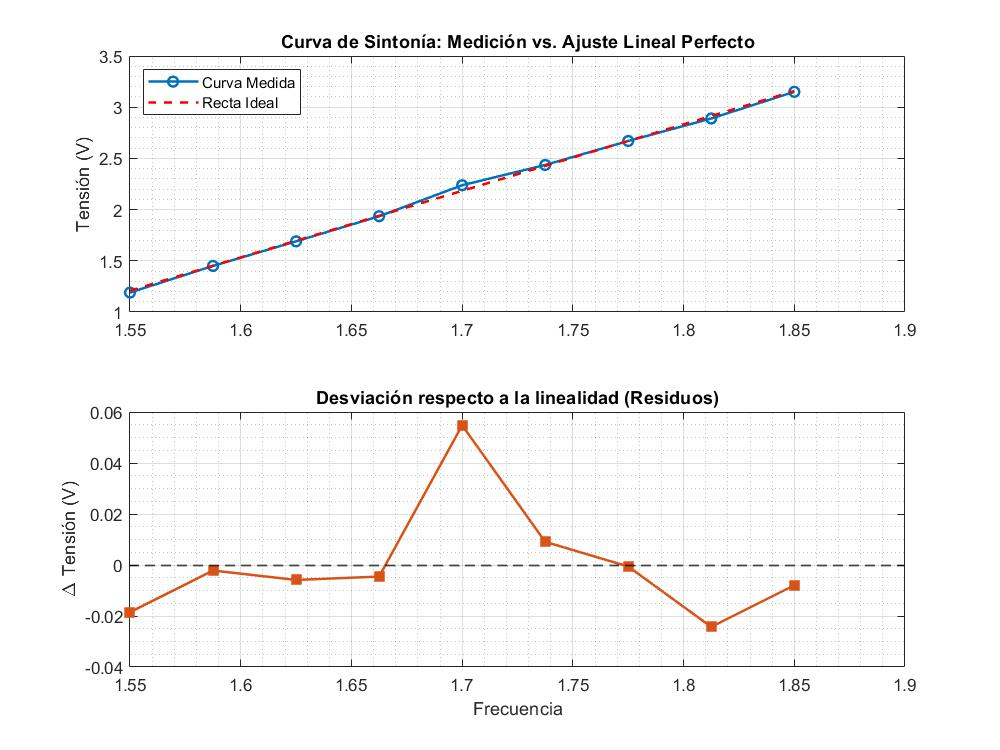
\includegraphics[width=\linewidth]{imagenes/rampanolinealyerror.jpg}
        \caption{Comparación entre rampa medida e ideal.}
        \label{fig:medicionrampa}
    \end{subfigure}
    \caption{Caracterización experimental del VCO a lazo abierto. (Fuente: Propia).}
    \label{fig:vco_mediciones_conjunto}
\end{figure}

\begin{table}[H]
\centering
\begin{tabular}{lcc}
\hline
\textbf{Parámetro} & \textbf{Hoja de datos / Diseño} & \textbf{Valor Medido} \\
\hline
Rango de frecuencia & $1550$ a $1850~\mathrm{MHz}$ & $1550$ a $1850~\mathrm{MHz}$ \\
Tensión de sintonización ($V_{\text{tune}}$) & $1{,}5~\mathrm{V}$ a $3{,}6~\mathrm{V}$ & $1{,}19~\mathrm{V}$ a $3{,}15~\mathrm{V}$ \\
Sensibilidad de sintonía ($K_V$) & $\approx 142{,}86~\mathrm{MHz/V}$ & $\approx 153{,}06~\mathrm{MHz/V}$ \\
\hline
\end{tabular}
\caption{Comparación entre especificaciones y valores medidos del VCO.}
\label{tab:resultados_vco}
\end{table}

A partir de las mediciones se determinó una sensibilidad de sintonía experimental de $153{,}06~\mathrm{MHz/V}$ y un nivel de espurios de $-32~\mathrm{dBc}$. Si bien la curva a lazo abierto presenta no linealidades intrínsecas, el dispositivo cubre de manera correcta el rango de frecuencia requerido, validando su comportamiento para ser integrado posteriormente al lazo de control cerrado del PLL.

\section*{Lazo de Enganche de Fase (PLL)}

La validación dinámica del lazo de enganche se llevó a cabo mediante la comparación directa entre la respuesta transitoria simulada en \textit{ADIsimPLL} y la tensión de control medida experimentalmente ante un salto de frecuencia de $1{,}55~\mathrm{GHz}$ a $1{,}85~\mathrm{GHz}$, ya que esta aporta gran información acerca de la respuesta de la función de transferencia a lazo cerrado.

En la Figura~\ref{fig:pll_lock_time_comparacion} se presentan de forma conjunta la simulación del tiempo de establecimiento (\textit{lock time}) y la respuesta temporal obtenida en el banco de pruebas.

\begin{figure}[H]
    \centering
    \begin{subfigure}[b]{0.48\linewidth}
        \centering
        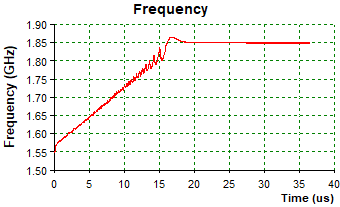
\includegraphics[width=\linewidth]{imagenes/adisimpll_lock_time.png}
        \caption{Simulación en ADIsimPLL.}
        \label{fig:adisimpll_lock_time_sec}
    \end{subfigure}
    \hfill
    \begin{subfigure}[b]{0.48\linewidth}
        \centering
        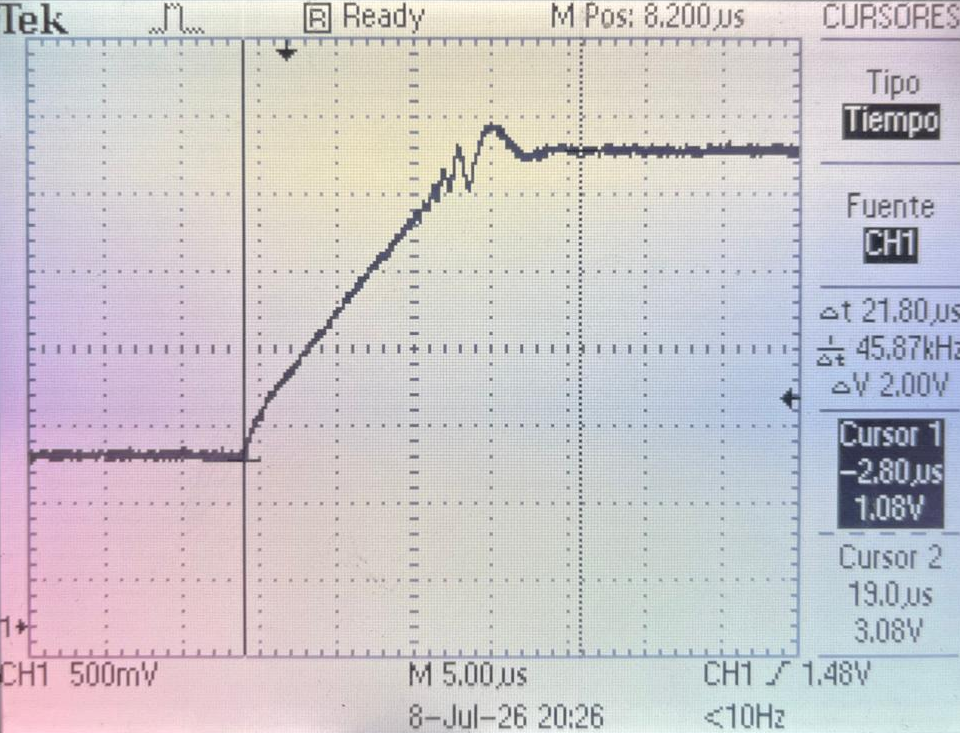
\includegraphics[width=\linewidth]{imagenes/medicion_1550_1850.png}
        \caption{Medición experimental de la tensión de control.}
        \label{fig:medicion_lock_time_sec}
    \end{subfigure}
    \caption{Comparación del tiempo de enganche del PLL entre simulación y medición experimental. (Fuente: Propia).}
    \label{fig:pll_lock_time_comparacion}
\end{figure}

Asimismo, con el propósito de caracterizar la estabilidad espectral y comprobar la mejora en la pureza de la señal al cerrar el lazo, se midió el ruido de fase del sistema integrado a frecuencia fija. La Figura~\ref{fig:ruido_fase_pll} muestra el perfil de ruido obtenido en el analizador.

\begin{figure}[H]
    \centering
    \begin{subfigure}[b]{0.48\linewidth}
        \centering
        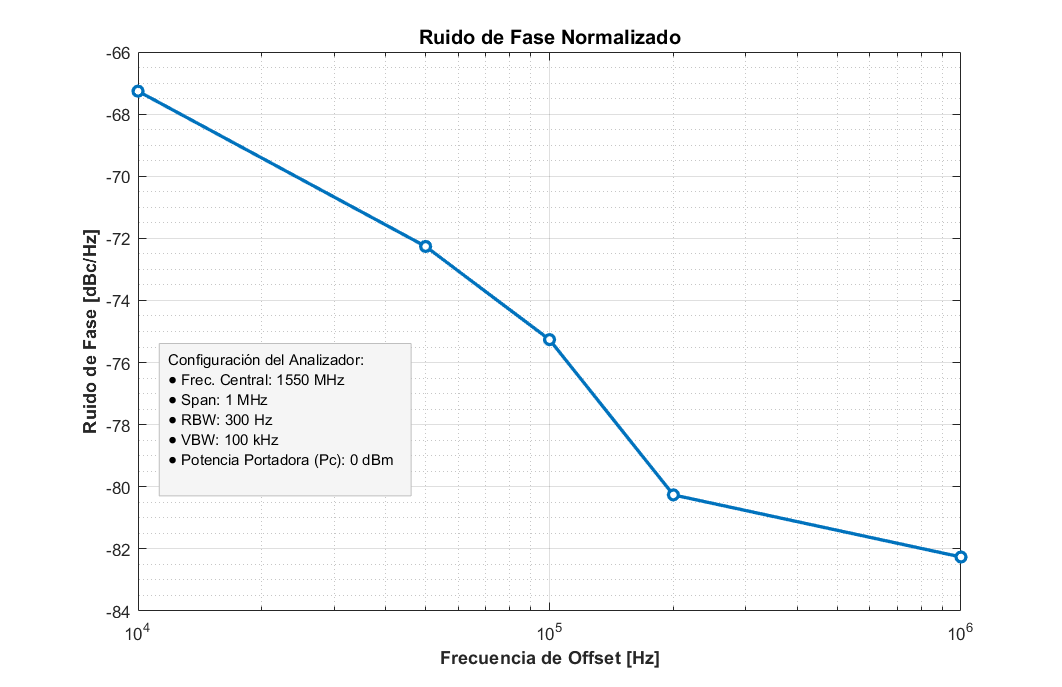
\includegraphics[width=\linewidth]{imagenes/ruido_fase_vco.png}
        \caption{Ruido de fase del VCO a lazo abierto.}
        \label{fig:ruido_fase_vco_solo}
    \end{subfigure}
    \hfill
    \begin{subfigure}[b]{0.48\linewidth}
        \centering
        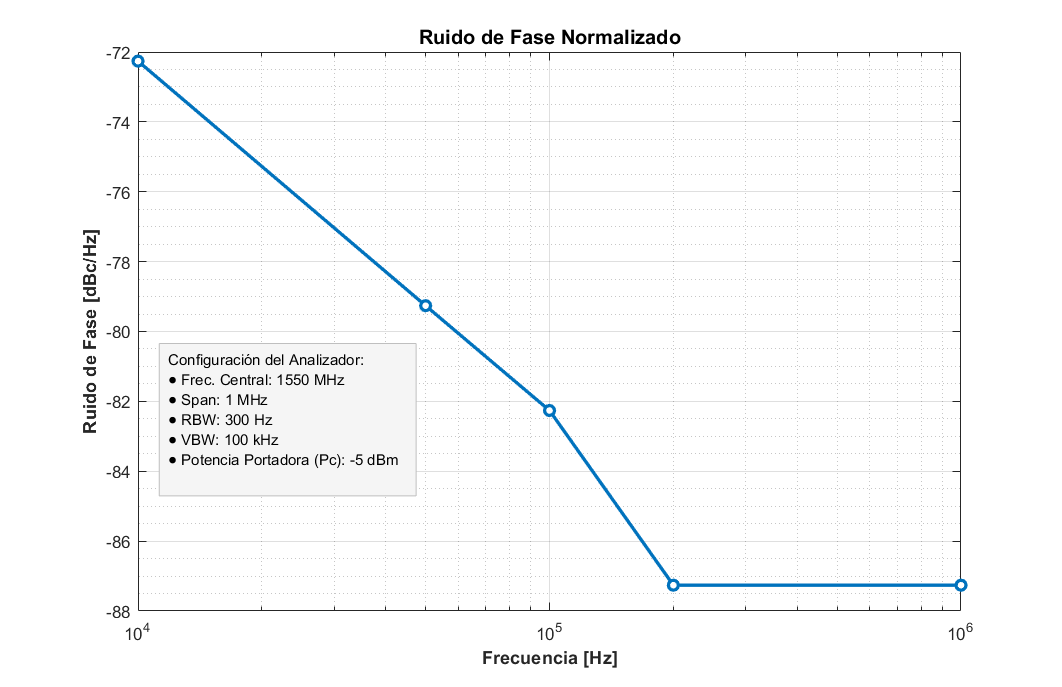
\includegraphics[width=\linewidth]{imagenes/ruido_fase_pll.png}
        \caption{Ruido de fase del sistema con PLL.}
        \label{fig:ruido_fase_pll_sistema}
    \end{subfigure}
    \caption{Comparación del ruido de fase entre el VCO libre y el sistema integrado con PLL a frecuencia fija. (Fuente: Propia).}
    \label{fig:ruido_fase_comparacion}
\end{figure}

\begin{table}[H]
\centering
\resizebox{\textwidth}{!}{%
\begin{tabular}{lcc}
\hline
\textbf{Parámetro} & \textbf{Simulado / Diseño} & \textbf{Valor Medido} \\
\hline
Ancho de banda del lazo ($BW$) & $\approx 290~\mathrm{kHz}$ & Verificado (dinámica acorde) \\
Margen de fase & $48^\circ$ & Estable \\
Tiempo de establecimiento (\textit{lock time}) & $\approx 20~\mu\mathrm{s}$ (pico: $16{,}2~\mu\mathrm{s}$) & $\approx 19~\mu\mathrm{s}$ (pico: $16{,}8~\mu\mathrm{s}$) \\
Mejora en ruido de fase (frente a VCO libre) & Reducción global & $-7~\mathrm{dBc}$ en promedio \\
\hline
\end{tabular}%
}
\caption{Comparación entre los parámetros teóricos/simulados y los resultados medidos del PLL.}
\label{tab:resultados_pll}
\end{table}

La respuesta temporal medida confirma una excelente concordancia con el modelo simulado en \textit{ADIsimPLL}, alcanzando un tiempo de establecimiento cercano a los $19~\mu\mathrm{s}$. Adicionalmente, el cierre del lazo logró reducir el ruido de fase en $7~\mathrm{dBc}$ en promedio respecto al oscilador libre, validando la estabilidad y el óptimo desempeño dinámico del sistema.


\section*{Barridos FMCW}

La evaluación del sistema completo bajo modulación FMCW se llevó a cabo configurando el sintetizador para generar rampas de frecuencia triangulares y en diente de sierra, cubriendo un ancho de banda total de $300~\mathrm{MHz}$ ($1{,}55~\mathrm{GHz}$ a $1{,}85~\mathrm{GHz}$).

En las Figuras~\ref{fig:fmcw_triangular} y \ref{fig:fmcw_sierra} se muestran las mediciones de los \textit{chirps} triangulares y de diente de sierra para los extremos de velocidad evaluados, junto con sus respectivas formas de onda de tensión de control en el osciloscopio. Asimismo, la Figura~\ref{fig:comparacion_rampas} presenta la comparación directa de las rampas generadas a diferentes velocidades.

\begin{figure}[H]
    \centering
    \begin{subfigure}[b]{0.48\linewidth}
        \centering
        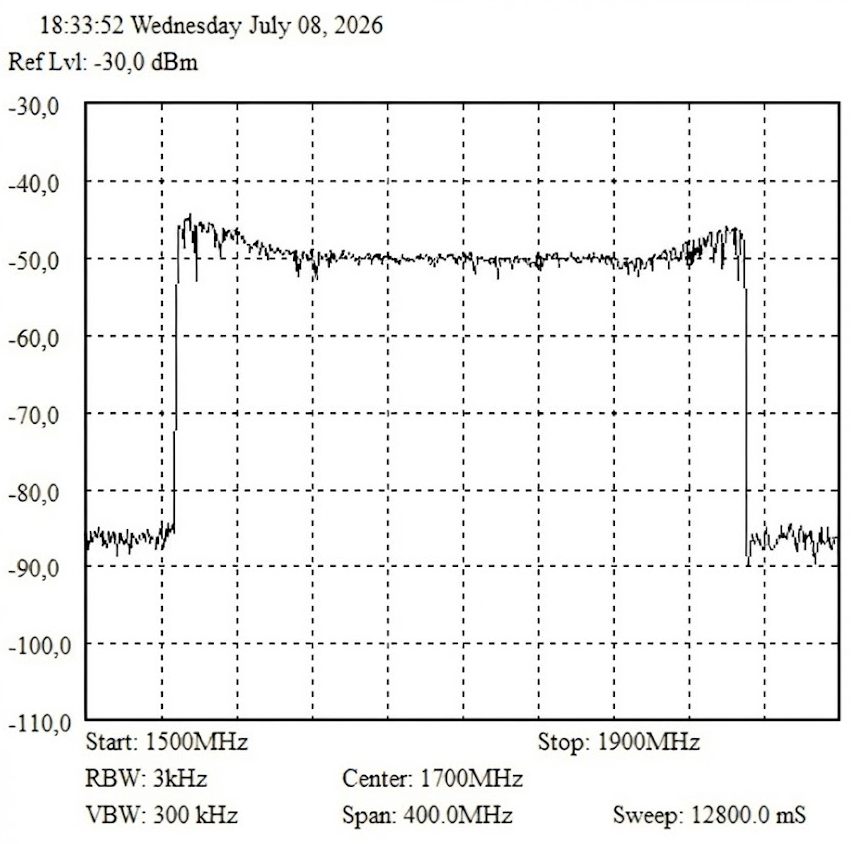
\includegraphics[width=\linewidth]{imagenes/chirp_1ms.png}
        \caption{Chirp triangular ($T = 1~\mathrm{ms}$).}
        \label{fig:fmcw_chirp_1ms}
    \end{subfigure}
    \hfill
    \begin{subfigure}[b]{0.48\linewidth}
        \centering
        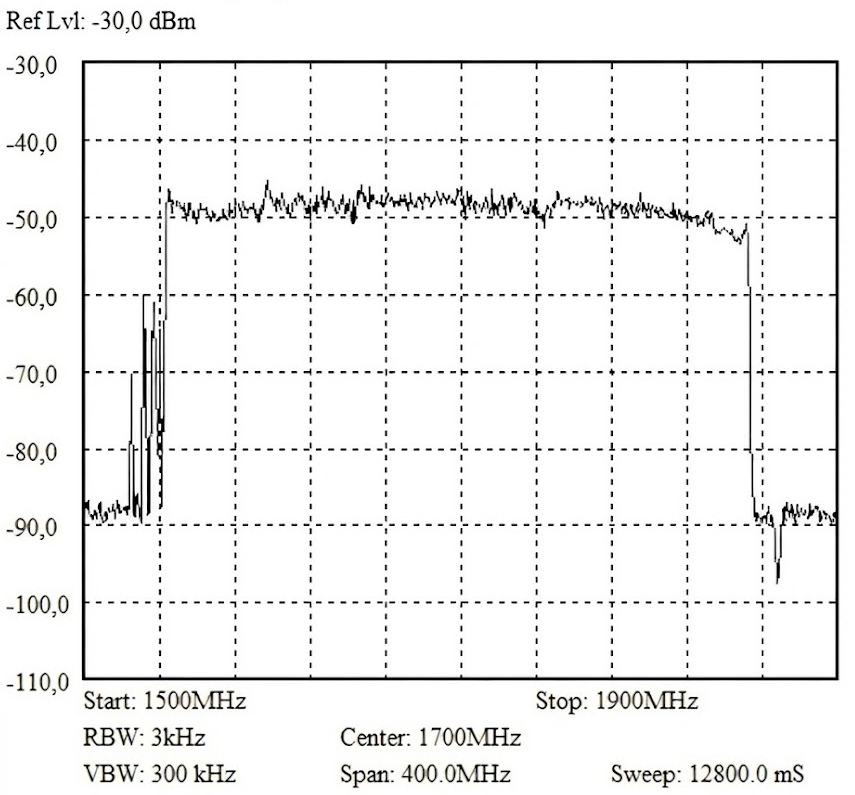
\includegraphics[width=\linewidth]{imagenes/chirp_002ms.png}
        \caption{Chirp triangular ($T = 0{,}02~\mathrm{ms}$).}
        \label{fig:fmcw_chirp_002ms}
    \end{subfigure}

    \vspace{0.3cm}

    \begin{subfigure}[b]{0.48\linewidth}
        \centering
        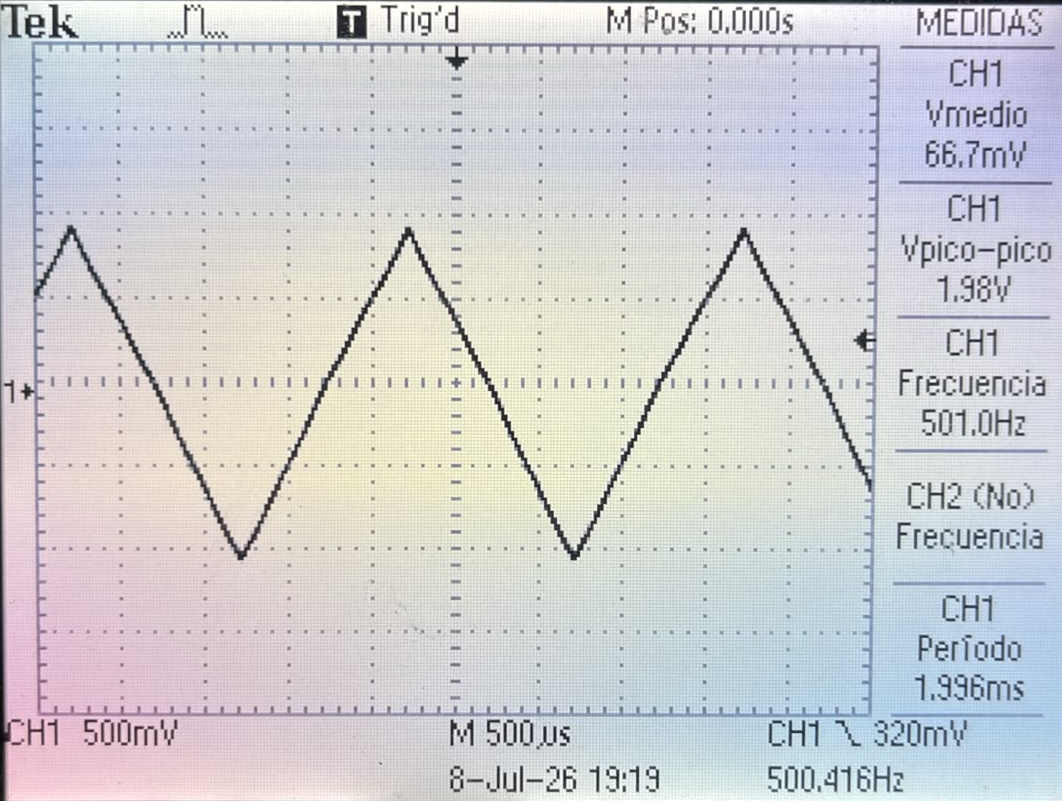
\includegraphics[width=\linewidth]{imagenes/tension_control1ms.png}
        \caption{Tensión de control ($T = 1~\mathrm{ms}$).}
        \label{fig:fmcw_tension_1ms}
    \end{subfigure}
    \hfill
    \begin{subfigure}[b]{0.48\linewidth}
        \centering
        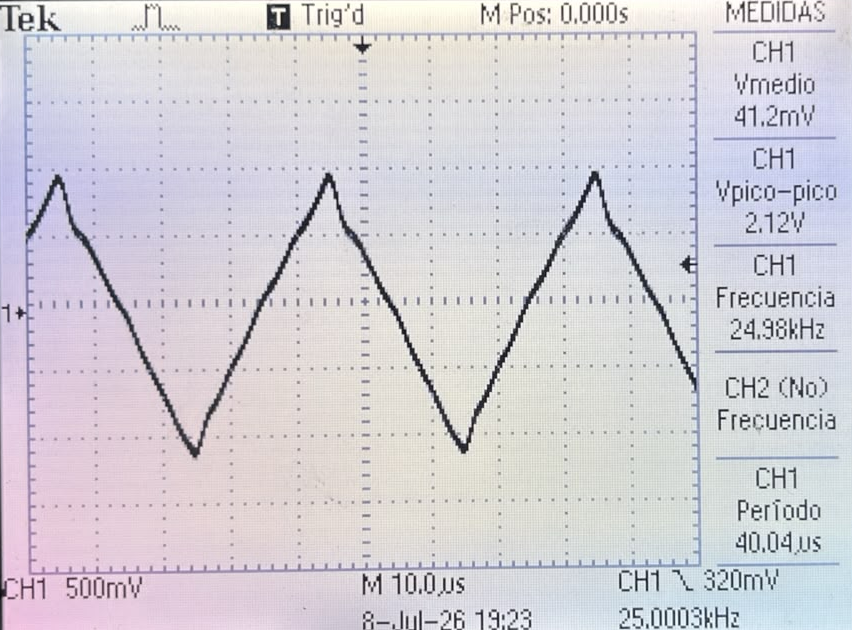
\includegraphics[width=\linewidth]{imagenes/tension_control002ms.png}
        \caption{Tensión de control ($T = 0{,}02~\mathrm{ms}$).}
        \label{fig:fmcw_tension_002ms}
    \end{subfigure}

    \caption{Mediciones experimentales para el perfil triangular en los extremos de velocidad. (Fuente: Propia).}
    \label{fig:fmcw_triangular}
\end{figure}

\begin{figure}[H]
    \centering
    \begin{subfigure}[b]{0.48\linewidth}
        \centering
        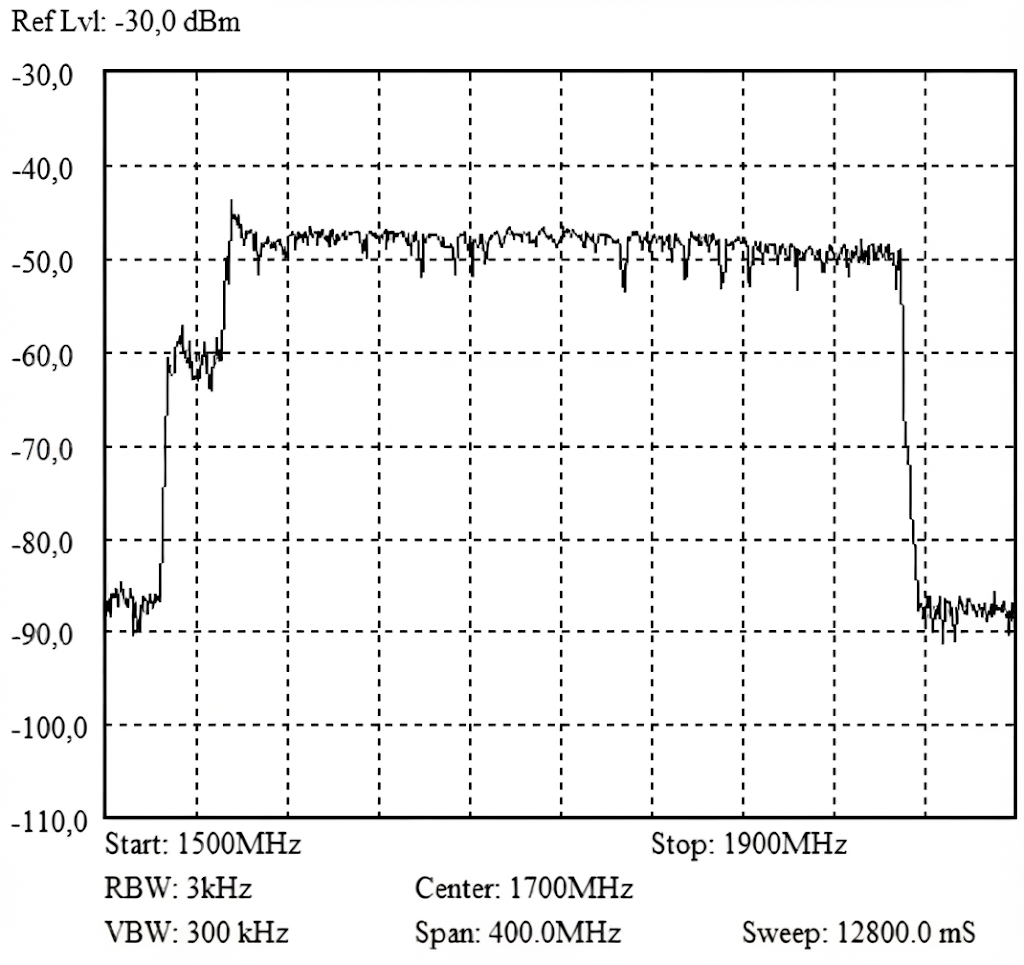
\includegraphics[width=\linewidth]{imagenes/chirp_sierra_1ms.png}
        \caption{Chirp diente de sierra ($T = 1~\mathrm{ms}$).}
        \label{fig:fmcw_sierra_1ms}
    \end{subfigure}
    \hfill
    \begin{subfigure}[b]{0.48\linewidth}
        \centering
        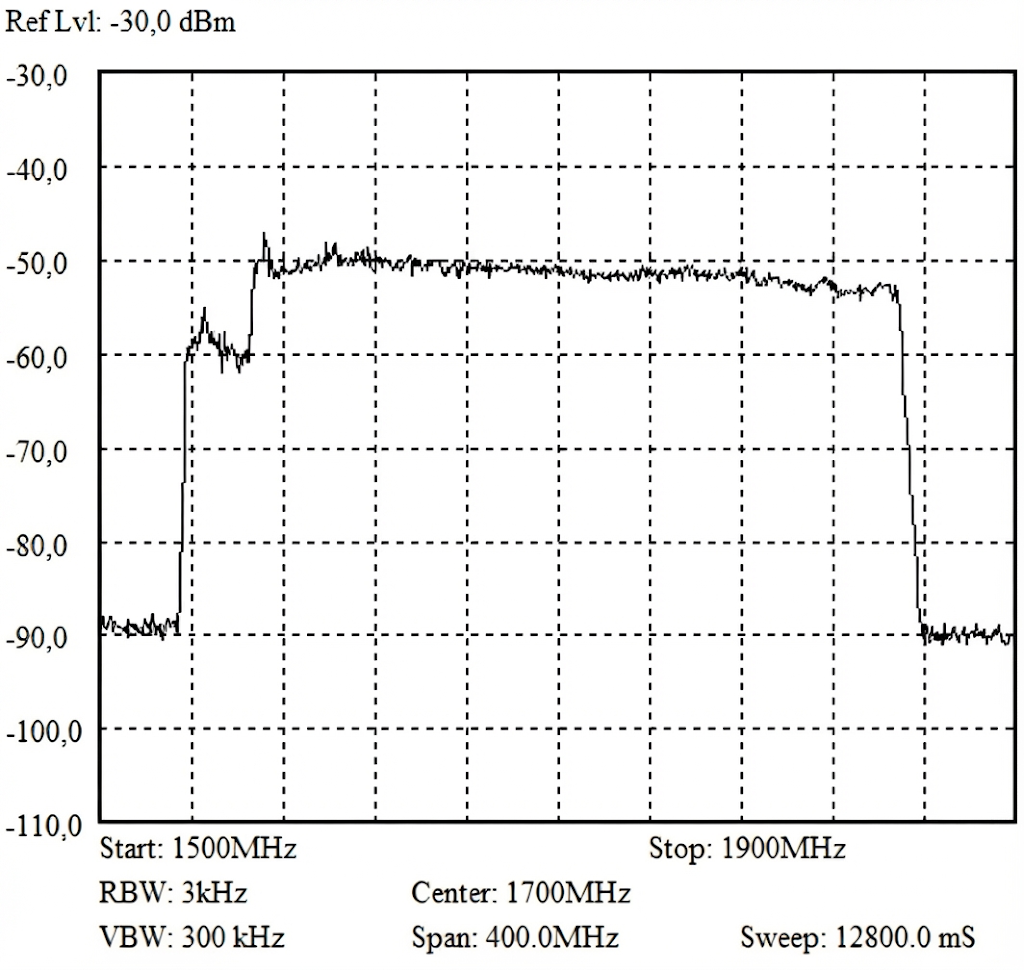
\includegraphics[width=\linewidth]{imagenes/chirp_sierra_025ms.png}
        \caption{Chirp diente de sierra ($T = 0{,}25~\mathrm{ms}$).}
        \label{fig:fmcw_sierra_025ms}
    \end{subfigure}

    \vspace{0.3cm}

    \begin{subfigure}[b]{0.48\linewidth}
        \centering
        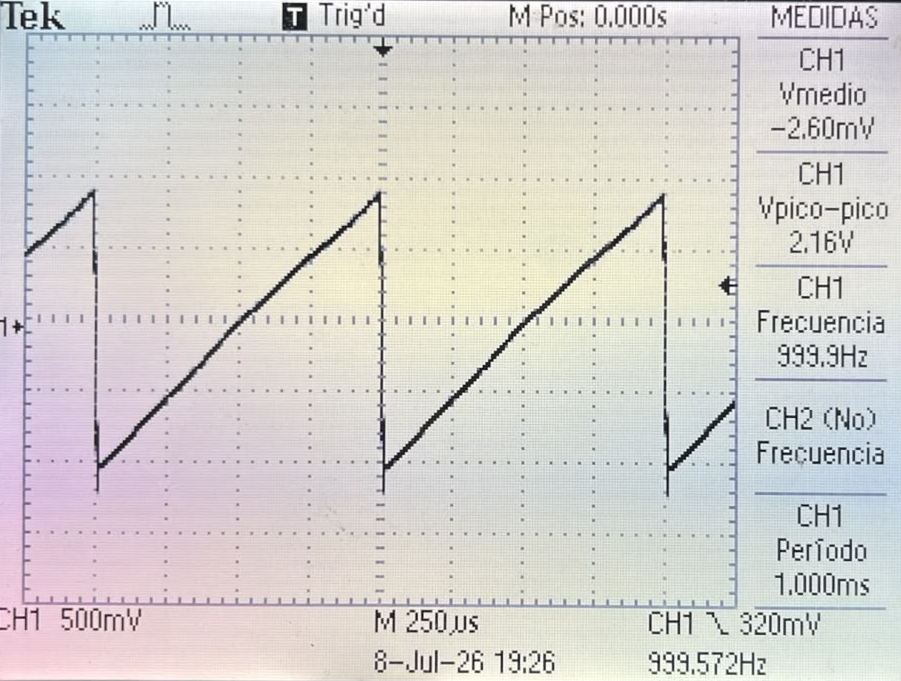
\includegraphics[width=\linewidth]{imagenes/tension_control_sierra1ms.png}
        \caption{Tensión de control ($T = 1~\mathrm{ms}$).}
        \label{fig:fmcw_tension_sierra_1ms}
    \end{subfigure}
    \hfill
    \begin{subfigure}[b]{0.48\linewidth}
        \centering
        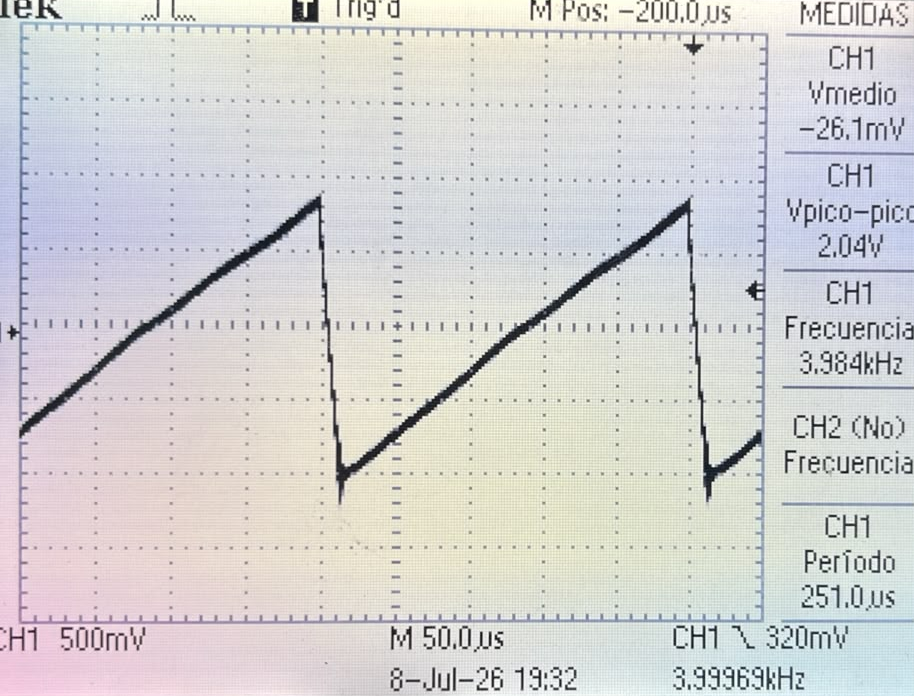
\includegraphics[width=\linewidth]{imagenes/tension_control_sierra025ms.png}
        \caption{Tensión de control ($T = 0{,}25~\mathrm{ms}$).}
        \label{fig:fmcw_tension_sierra_025ms}
    \end{subfigure}

    \caption{Mediciones experimentales para el perfil diente de sierra en los extremos operativos. (Fuente: Propia).}
    \label{fig:fmcw_sierra}
\end{figure}

\begin{figure}[H]
    \centering
    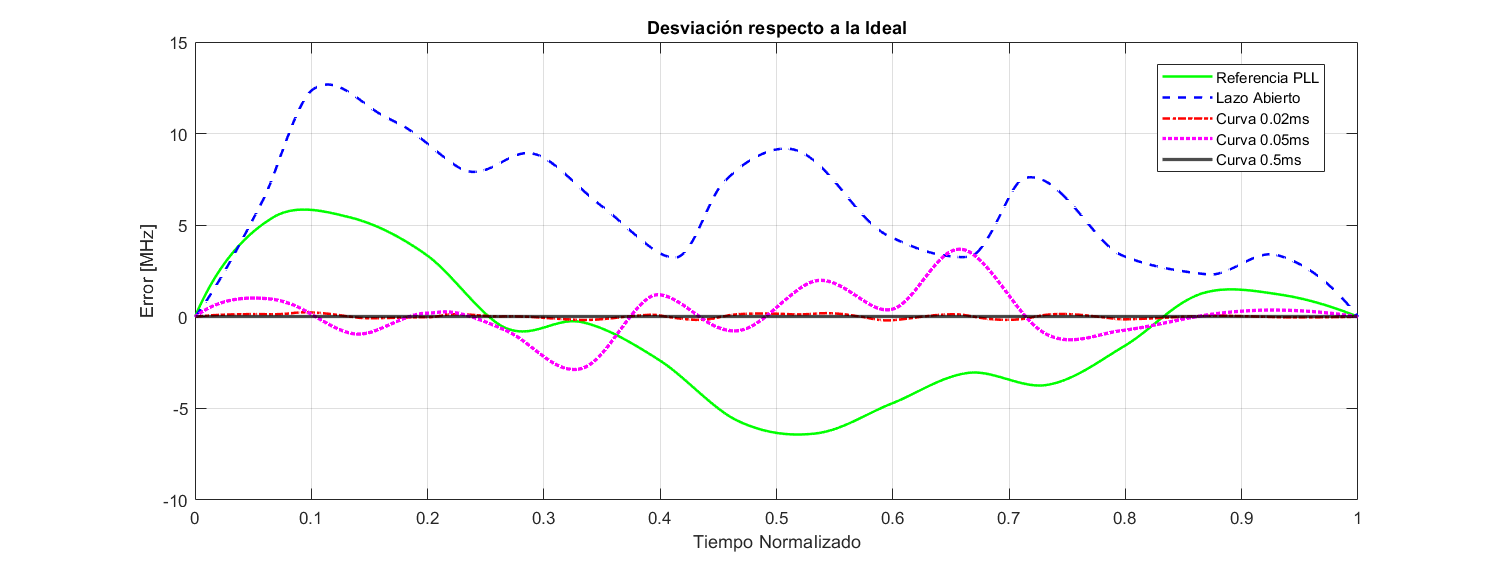
\includegraphics[width=0.85\linewidth]{imagenes/comparaciónrampas.png}
    \caption{Comparación de las rampas de frecuencia generadas para tiempos de barrido de $0{,}5~\mathrm{ms}$, $0{,}05~\mathrm{ms}$ y $0{,}02~\mathrm{ms}$. (Fuente: Propia).}
    \label{fig:comparacion_rampas}
\end{figure}

\begin{table}[H]
\centering
\resizebox{\textwidth}{!}{%
\begin{tabular}{lcccc}
\hline
\textbf{Tiempo de barrido ($T$)} & \textbf{Ancho de banda} & \textbf{Desviación máxima} & \textbf{Linealidad / Desempeño} \\
\hline
$1~\mathrm{ms}$ (Triangular) & $300~\mathrm{MHz}$ & $150~\mathrm{kHz}$ & Mejor linealidad del lazo \\
$0{,}5~\mathrm{ms}$ (Triangular) & $300~\mathrm{MHz}$ & $240~\mathrm{kHz}$ & Óptimo rendimiento dinámico \\
$0{,}05~\mathrm{ms}$ (Triangular) & $300~\mathrm{MHz}$ & $2{,}5~\mathrm{MHz}$ & Incremento de la no linealidad del lazo \\
$0{,}02~\mathrm{ms}$ (Triangular) & $300~\mathrm{MHz}$ & $13{,}5~\mathrm{MHz}$ & Error grande de linealidad \\
$1~\mathrm{ms}$ (Diente de sierra) & $300~\mathrm{MHz}$ & $150~\mathrm{kHz}$ & Lineal en rampa ascendente, gran sobrepasamiento \\
\hline
\end{tabular}%
}
\caption{Resumen de resultados experimentales para diferentes perfiles y tiempos de barrido FMCW.}
\label{tab:resultados_fmcw}
\end{table}

A partir de las mediciones se comprueba que para tiempos de barrido moderados ($0{,}5~\mathrm{ms}$) el PLL sigue fielmente la modulación impuesta con una desviación inferior a $240~\mathrm{kHz}$. Al incrementar la velocidad ($0{,}05~\mathrm{ms}$ y $0{,}02~\mathrm{ms}$), las limitaciones dinámicas del lazo introducen desviaciones significativas de hasta $13{,}5~\mathrm{MHz}$. Por otro lado, las modulaciones de diente de sierra presentan un comportamiento similar en el barrido, pero agregan un error asociado al sobrepasamiento; este efecto se puede mitigar mediante el uso de una segunda rampa de bajada (\textit{Fast ramp}) que suaviza la caída de la señal e introduce una modificación en el período total de la onda. Este modo de funcionamiento logra disminuir el sobrepasamiento de $40~\mathrm{MHz}$ a $5~\mathrm{MHz}$.